\chapter{Experimentální část}

%%%%%%%%%%%%%%%%%%%%%%%%%%%%%%%%%%%%%%%%%%%%%%%%%
\section{Analýza}

% popis Manty
\subsection{Manta Flow}
\textit{Manta Flow}\footnote{https://getmanta.com/} je nástroj umožňující automatickou analýzu zdrojového kódu (SQL, Java) a následný popis transformační logiky v něm obsažené. Software je schopný rozpoznat i těžce čitelné konstruky zdrojového kódu. Díky tomu dokáže automaticky zanalyzovat rozsáhlé databáze a vytvořit z nich přehlednou mapu datových toků, neboli \textit{Data Lineage}. To se v praxi využívá převážně k optimalizaci datových skladů, snižování nákladů na vývoj softwaru, provádění dopadových analýz a při dokumentování prostředí pro potřeby regulačních úřadů.

Nástroj má dvě hlavní komponenty (viz diagram \ref{fig:ana-flow-comp}): 
\begin{itemize}
	\item{\textit{Manta Flow CLI}}: je Java řádková aplikace provádějící extrakci skriptů ze zdrojových databází a uložišť a jejich analýzu. Analyzovaná data jsou následně poslána \textit{Manta Flow Serveru}. \textit{Klientská aplikace} také může nahrávat vygenerované exporty ze \textit{serveru} do externí metadatové databáze. 
	\item{\textit{Manta Flow Server}}: je serverová Java aplikace, která ukládá získané informace do interního metadatového uložiště, transformuje je, umožňuje jejich visualizaci a přístup k nim pomocí veřejného API. 
\end{itemize}

Interakce mezi \textit{klientskou} a \textit{serverovou} částí aplikace je popsána zjednodušeným sekvenčním diagramem \ref{fig:ana-flow-seq}. 

\begin{figure}
\begin{center}
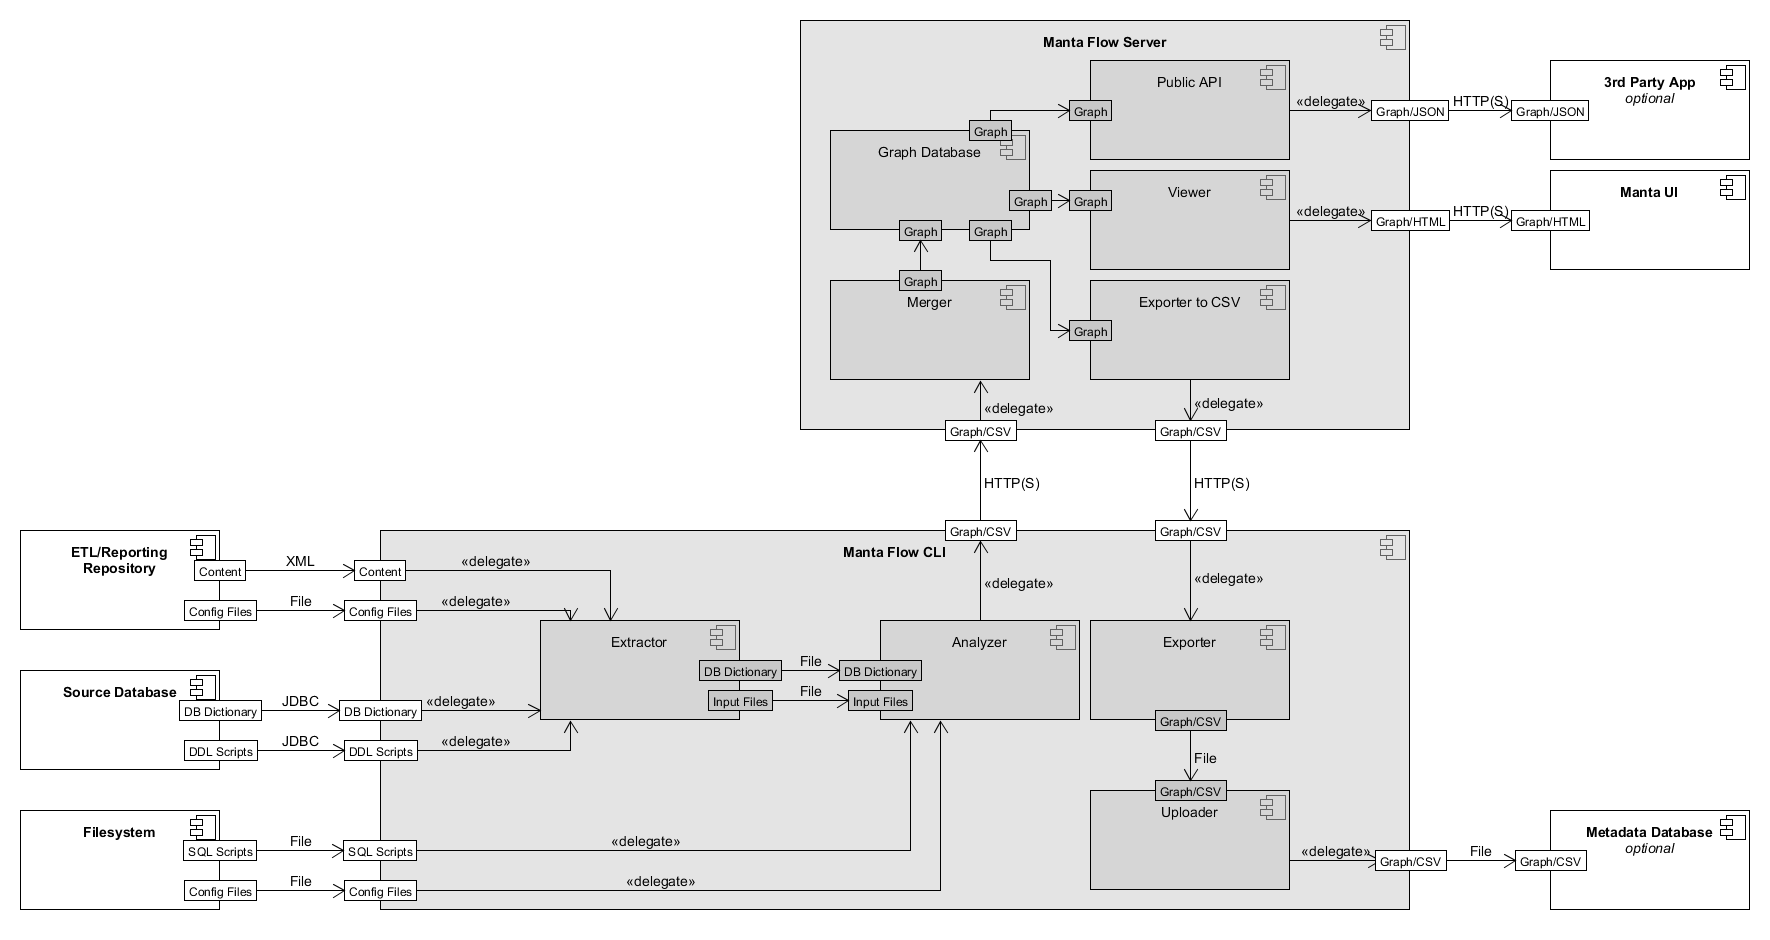
\includegraphics[width=14cm]{figures/flow_comp}
\caption{Architektura \textit{Manta Flow}}
\label{fig:ana-flow-comp}
\end{center}
\end{figure}

\begin{figure}
\begin{center}
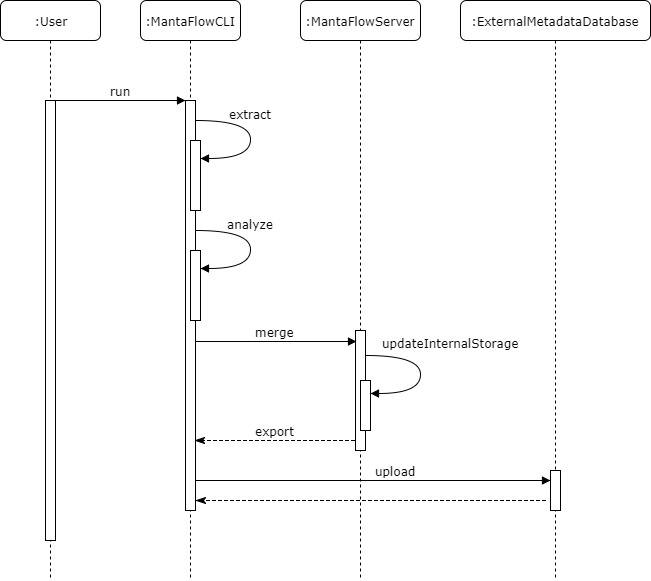
\includegraphics[width=14cm]{figures/flow_seq}
\caption{Interakce mezi \textit{klientskou} a \textit{serverovou} částí \textit{Manta Flow}}
\label{fig:ana-flow-seq}
\end{center}
\end{figure}

\subsection{Metadatové uložiště}
Jak již bylo zmíněno v úvodu práce (kapitola \ref{sec:uvod}) metadatové uložiště produktu \textit{Manta Flow} je aktuálně implementováno grafovou databází \textit{Titan} (ve verzi 0.4) a je snaha o výměnu této databáze %\cite{TODO Kovar}. 
Než přistoupíme k bližšímu popisu jednotlivých komponent aplikace a jejich interakcí s metadatovým uložištěm (kapitola \ref{sec:ana_interactions}, je třeba nejdříve popsat jeho datový model zobrazený na obrázku \ref{fig:ana-model}. 

% TODO popsat reálné entity 

\begin{figure}
\begin{center}
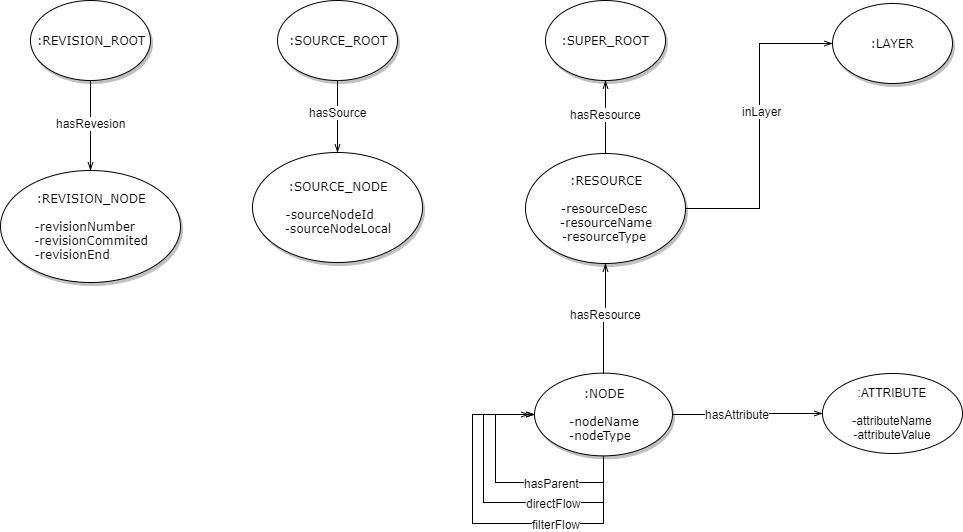
\includegraphics[width=14cm]{figures/model}
\caption{Model grafové databáze}
\label{fig:ana-model}
\end{center}
\end{figure}

Model se skládá z devíti typů uzlů:

\begin{itemize}
	\item{\textit{SUPER\_ROOT}}: Uzel (právě jeden v databázi), který slouží jako umělý kořen všech uzlů typu \textit{RESOURCE}. 
	\item{\textit{RESOURCE}}: Uzly tohoto typu reprezentují zdrojové systémy - zdroje definic objektů, zdrojových kódů, ETL řešení a další.  
	\item{\textit{NODE}}: Uzly typu \textit{NODE} představují reálné objekty zdrojového systému - databáze, tabulky, sloupce, procedury, skripty a další. 
	\item{\textit{LAYER}}: Uzly typu \textit{LAYER} reprezentují vrstvy modelu metadat. Datové toky nalezené při analýze zdrojových kódů jsou vždy ukládány do \textit{fyzické vrstvy}, ze které je potom možné generovat abstraktnější vrstvy modelu datových toků.  
	\item{\textit{ATTRIBUTE}}: Uzly typu \textit{ATTRIBUTE} reprezentují atributy uzlů typu \textit{NODE} - parametry sloupců, popisy databázových objektů a další.
	\item{\textit{SOURCE\_ROOT}}: Uzel (právě jeden v databázi), který slouží jako umělý kořen všech uzlů typu \textit{SOURCE\_NODE}. 
	\item{\textit{SOURCE\_NODE}}: Uzly typu \textit{SOURCE\_NODE} reprezentují soubory se zdrojovými kódy extrahovanými ze zdrojových systémů. 
	\item{\textit{REVISION\_ROOT}}: Uzel (právě jeden v databázi), který slouží jako umělý kořen všech uzlů typu \textit{REVISION\_NODE}. 
	\item{\textit{REVISION\_NODE}}: Uzly typu \textit{ATTRIBUTE} reprezentují revize modelu metadat, definují tedy jeho verzování. Kromě dalších parametrů mají všechny hrany grafu parametry \textit{tranEnd} a \textit{tranStart} definující platnost hran (viz obrázek \ref{fig:ana-model-rev}). Při každé analýze zdrojových systémů (která je prováděna dávkově klientskou částí aplikace) je vytvořena nová revize metadatového uložiště obsahující všechny objekty zdrojových systémů.\footnote{Je snaha tento princip upravit tak, aby byly objekty v metadatovém uložišti minimálně repklikovány \cite{Sykora17}.}  
\end{itemize}

 a osmi typů hran:

 \begin{itemize}
	\item{\textit{hasResource}}: Hrana přiřazuje objekty (uzly typu \textit{NODE}) ke svým zdrojovým systémům (uzlům typu \textit{RESOURCE}). Hrana je také použite k propojení uzlů typu \textit{RESOURCE} s uzlem \textit{RESOURCE\_ROOT}.
	\item{\textit{hasParent}}: Hrana mezi dvěmi uzly typu \textit{NODE} vytvářející klasickou hiearchickou strukturu mezi těmito uzly - strom závislostí objektů zdrojových systémů. 
	\item{\textit{directFlow}}: Hrana mezi dvěmi uzly typu \textit{NODE} říkající, že mezi těmito uzly existuje přímý datový tok (ve směru hrany).
	\item{\textit{filterFlow}}: Hrana mezi dvěmi uzly typu \textit{NODE} říkající, že mezi těmito uzly existuje nepřímý datový tok (ve směru hrany).
	\item{\textit{hasAttribute}}: Hrana přiřazující uzlům typu \textit{NODE} jejich atributy (uzly typu \textit{ATTRIBUTE}).
	\item{\textit{inLayer}}: Hrana typu \textit{inLayer} spojeju zdroje (uzly typu \textit{RESOURCE}) a vrstvy a říká, že zdroj patří do dané vrstvy modelu metadat. 
	\item{\textit{hasSource}}: Hrana je použita k propojení uzlů reprezentujících zdrojové kódy (uzly typu \textit{SOURCE\_NODE}) s uzlem \textit{SOURCE\_ROOT}.
	\item{\textit{hasRevision}}: Hrana je použita k propojení uzlů reprezentujících revize modelu metadat (uzly typu \textit{REVISION\_NODE}) s uzlem \textit{REVISION\_ROOT}.
\end{itemize}

\begin{figure}
\begin{center}
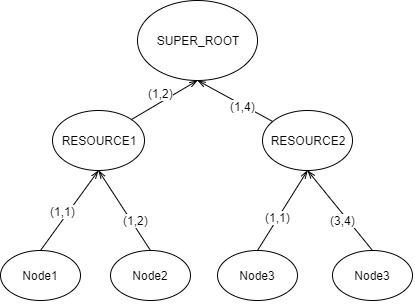
\includegraphics[width=6cm]{figures/model_revisions}
\caption{Způsob verzování modelu metadat}
\label{fig:ana-model-rev}
\end{center}
\end{figure}

% TODO indexy

\subsection{Interakce s metadatovým uložištěm}
\label{sec:ana_interactions}
%TODO bližší popis jednotlivých feature souvisejících s GDB
% TODO

% Merger
% Otázky
%  - co vše obsahuje jeden mergovaný graf? 
%  - co je scriptmetadata? 

% Vstup - serializovaný graf - byte[]
% Merge se provádí buď do nové verze, nebo pokud je verzování vypnuto do HEAD_REVISION

% merge s VCS on 
% - check
%  - transakce - WRITE_SHARE (paralel) / WRITE_EXCLUSIVE (serial) -- u serialu je to ale zbytečné, ne? :) 
%  - checkMergeConditions (pouze najde revision node a zjistí, jestli revize existuje (jak byla vytvořena?) a není commitnutá)
% - processor.process 
%  - transakce - WRITE_SHARE (paralel) / WRITE_EXCLUSIVE (serial) -- u serialu je to ale zbytečné, ne? :) 
%  - vloží SOURCE uzly do db a pokud je vypnuto verzování, zkontroluje počet proti licenci
%   - transakce
%   - kazdy skript - scriptMetadataDao.create/update  --- @Insert("INSERT INTO script_metadata (script_hash, last_processin...    ---- takže co je skript metadata?
%   - podmínečný commit (počet skriptů vs licence)
%  - mergne objekty (každý má vlastní merge metodu) a občas udělá commit (podle počtu nových objektůs)
%					TitanVertexQuery query = ((TitanVertex) parentVertex).query()
%                    .has(EdgeProperty.CHILD_NAME.t(), GraphOperation.processValueForChildName(name))
%                    .has(EdgeProperty.TRAN_END.t(), Cmp.GREATER_THAN_EQUAL, lastCommitedRevision)
%                    .direction(Direction.IN).labels(parentEdgeType.t());
%   - pokud uzel není ve výsledku dotazu, je vytvořen (jinak nic)  ---- public static Vertex createNode(TitanTransaction transaction, Vertex parent, String name, String type,
%            Integer revision)
% merge bez VCS je stejný, akorát processor.process neběží v transakci

% TODO 
% Query

% TODO 
% Viewer

% TODO
% Public API

% TODO 
% Export to CSV

% TODO POPIS API jednotlivých databází
\subsection{GDB API} %TODO CHANGE

%TODO
\subsection{Požadavky}


